\chapter{Introduction}\label{intro}
\section{Motivation}
A \acrfull{bg} is a graph with two disjoint vertex sets where its edges only connect vertices from different sets. 
For instance, two different sets of objects can be modeled with a \acrshort{bg}, establishing the relationships between them.
There are different use cases in which we can take advantage of a \acrshort{bg} representation and detect how the elements between the sets
are related. For example in coding theory~\cite{DBLP:journals/corr/WangL13} has been studied to represent relation between words in code 
or for representing graphs in hypergraph theory~\cite{hypergraph}. Another important field that we consider this has a strong potential is 
in pharmacology, where the relation between the drugs and side effects can be modeled with \acrshort{bg} as well~\cite{drugs}.

In order to detect the underlying relations of the different sets components in a \acrshort{bg} we have at our disposal the same metrics as \acrfull{ug}.
Unfortunately most of those metrics on \acrshort{ug} like clustering coefficient, social analysis or triangle-based community computation~\cite{ccoef,detect_graph,Newman_2003},
are based on computing the number of triangles in the network. Obtaining those metrics on \acrshort{bg} requires to count \acrfull{bt} on \acrshort{bg}.
In that matter, there has been a novel work that provides efficient algorithms to count \acrshort{bt} in $P$~\cite{btcount}.

On the other hand, there exists other kind of relationships in \acrshort{bg} that cannot be obtained only by counting \acrshort{bt} and requires to know specific
structural details about those \acrshort{bt}. One of those relations are motif-paths~\cite{Li2019MotifPA}, in particular a \acrshort{bt} is a motif and for detecting
a path between different \acrshort{bt} we need to be able to enumerate the \acrshort{bt} more than counting.
Moreover, in large \acrshort{bg} with millions of \acrshort{bt} an user might want to not wait for enumerating all the \acrshort{bt} that are participating on the network,
and it might require to ask for some of them that matches certain characteristics, like in motif-path semantic. This leads us to the main motivation of this work which is provide
an incremental algorithm to enumerate \acrlong{bt} in \acrlong{bg}.

Regarding the possible implementations of this kind of algorithm, streaming processing has given rise to new computation paradigms to provide effective and efficient data stream processing.
The most important features of these new paradigms are the exploitation of parallelism, the capacity to adapt execution schedulers, 
reconfigure computational structures, adjust the use of resources according to the characteristics of the input stream and produce incremental results. 
The \acrfull{dp} is a naturally functional approach to deal with stream processing. 
This fact encourages us to use \acrlong{hs}, a purely functional programming language, for \acrshort{dp}.

In conclusion, taking advantage of this computational model we can design an incremental algorithm to enumerate \acrshort{bt} in \acrshort{bg}.

\section{Problem Statement}
Before presenting the problem statement we should provide some definitions.

\begin{definition}[\acrlong{bg}] 
A bipartite graph is an undirected graph $G=(V,E)$  such that $V=(U\cup L)$, $U\cap L=\emptyset$ and $E\subseteq U\times L$.\cite{Bondy1976}
\end{definition}

Since the bipartite graph $G$ is an undirected graph, the edges in $E$ are bidirectional and although $E\subseteq U\times L$, in an abuse of notation, we indistinctly use $(u,l)$ and $(l,u)$ for edges in $E$. Additionally, 
without loss of generality, we assume that  $U\subseteq \mathbb{N}$ and $L\subseteq \mathbb{N}$. Consequently, $(U,<)$  and $(L,<)$ are strict total orders. We can see an example of a \acrshort{bg}
in \autoref{fig:bipartite-graph-example}.

\begin{figure}[h]
	\centering	
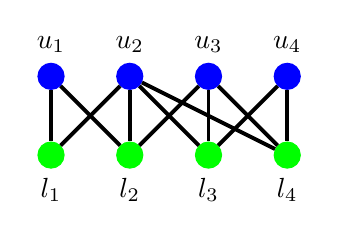
\begin{tikzpicture}
 \node[shape=circle,draw=blue,fill=blue,label=above:$u_1$] (u1) {};
 \node[shape=circle,draw=blue,fill=blue,label=above:$u_2$] (u2) [right of=u1] {};
 \node[shape=circle,draw=blue,fill=blue,label=above:$u_3$] (u3) [right of=u2] {};
 \node[shape=circle,draw=blue,fill=blue,label=above:$u_4$] (u4) [right of=u3] {};
 \node[shape=circle,draw=green,fill=green,label=below:$l_1$] (l1) [below of=u1] {};
 \node[shape=circle,draw=green,fill=green,label=below:$l_2$] (l2) [below of=u2] {};
 \node[shape=circle,draw=green,fill=green,label=below:$l_3$] (l3) [below of=u3] {};
 \node[shape=circle,draw=green,fill=green,label=below:$l_4$] (l4) [below of=u4] {};

 \draw (u1) [line width=0.5mm] -- (l1);
 \draw (u1) [line width=0.5mm] -- (l2);
 \draw (u2) [line width=0.5mm] -- (l1);
 \draw (u2) [line width=0.5mm] -- (l2);
 \draw (u2) [line width=0.5mm] -- (l3);
 \draw (u2) [line width=0.5mm] -- (l4);
 \draw (u3) [line width=0.5mm] -- (l2);
 \draw (u3) [line width=0.5mm] -- (l3);
 \draw (u3) [line width=0.5mm] -- (l4);
 \draw (u4) [line width=0.5mm] -- (l3);
 \draw (u4) [line width=0.5mm] -- (l4);
\end{tikzpicture}

\caption{Example of \acrshort{bg}}
\label{fig:bipartite-graph-example}
\end{figure}

 

%
\begin{definition}[\acrlong{bt}]
Let $G=((U\cup L),E)$ be a bipartite graph. Let the triples $\mu=(u_1, u_2, u_3)$ and $\ell=(l_1, l_2,l_3)$ on $U$ and $L$, respectively, i.e.  $\{u_1, u_2, u_3\} \subseteq U$, $\{l_1, l_2,l_3\} \subseteq L$. 
The 6-cycle $u_1,l_1,u_2,l_3,u_3,l_2,u_1$  is a \textit{bi-triangle} in $G$, denoted by $BT_{\ell}^{\mu} = \bti$. 
\end{definition}

In what follows, when convenient, the bi-triangle $BT_{(l_1,l_2,l_3)}^{(u_1,u_2,u_3)}$  will be denoted by the set of edges $\{(u_1, l_1), (l_1,u_2), (u_2, l_3), (l_3,u_3), (u_3, l_2), (l_2,u_1)\} \subseteq E$

\begin{figure}[h]
	 \centering	
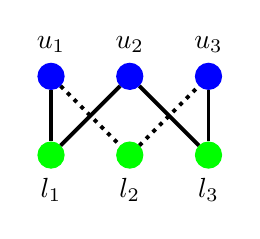
\begin{tikzpicture}
	\node[shape=circle,draw=blue,fill=blue,label=above:$u_1$] (1) {};
	\node[shape=circle,draw=blue,fill=blue,label=above:$u_2$] (2) [right of=1] {};
	\node[shape=circle,draw=blue,fill=blue,label=above:$u_3$] (3) [right of=2] {};
	\node[shape=circle,draw=green,fill=green,label=below:$l_1$] (4) [below of=1] {};
	\node[shape=circle,draw=green,fill=green,label=below:$l_2$] (5) [below of=2] {};
	\node[shape=circle,draw=green,fill=green,label=below:$l_3$] (6) [below of=3] {};

	\draw (1) [line width=0.5mm] -- (4);
	\draw (1) [dotted,line width=0.5mm] -- (5);
	\draw (4) [line width=0.5mm] -- (2);
	\draw (5) [dotted,line width=0.5mm] -- (3);
	\draw (6) [line width=0.5mm] -- (3);
	\draw (6) [line width=0.5mm] -- (2);
\end{tikzpicture}

\caption{Example of \acrshort{bt} in \acrshort{bg}}
\label{fig:bitriangle-example}
\end{figure}

	

In \autoref{fig:bitriangle-example} we can see a correct \acrshort{bt} in a \acrshort{bg}, and in the other \autoref{fig:bitriangle-not} we can see what it is not a \acrshort{bt}.

\begin{definition}[Query]
Let $G=((U\cup L),E)$ be a bipartite graph. 
A \textit{query} $Q$ is a sum type $Q = Q_V + Q_E$, where $Q_V \subseteq (U \cup L)$ and $Q_E \subseteq E$. 
It could be a query of vertices or edges.
\end{definition}

\begin{definition}[Query Match]
  Let $G=((U\cup L),E)$ be a bipartite graph.
  Let $Q$ be a query.
  A query $Q$ matches in a bipartite graph $G$ if forall $BT_{(l_1,l_2,l_3)}^{(u_1,u_2,u_3)}$ of $G$
  \[
    Q = \left\{\begin{array}{lr}
      Q_V, & \forall\ v \in Q_V, v \in \{l_1,l_2,l_3,u_1,u_2,u_3\}\\
      Q_E, & \forall\ (u,l) \in Q_E, (u,l) \in \{(u_1, l_1), (l_1,u_2), (u_2, l_3), (l_3,u_3), (u_3, l_2), (l_2,u_1)\} 
      \end{array}\right\} 
  \]
  \end{definition}
  
\paragraph{Statement:}Given a \acrlong{bg} $G$ and a query $Q$, incrementally enumerate all the \acrlong{bt} $BT_{\ell}^{\mu}$ that matches query $Q$.

\section{Proposed Solution}
The solution proposed in this work is implementing this algorithm using \acrfull{dp} implemented in \acrfull{hs}.
In that propose, we first develop a \acrlong{dpf} written in \acrlong{hs} that could help to implement any algorithm using \acrshort{dp}.
Following that, we provide a correct pseudo-code algorithm for incrementally enumerate \acrshort{bt} using \acrshort{dp}. And finally, we  
show the implementation of that pseudo-code using the \acrshort{dpf} in \acrshort{hs}, that we call \acrfull{dpbt}.

\section{Contribution}\label{sec:contrib}
One of the main contributions made, during the research of the present work, was the presentation of a paper in the \acrfull{prole21} Conference~\cite{prole21}. 
On the first hand, the motivation that trigger this contribution was first to asses the suitability of \acrshort{hs} to implement \acrshort{dp}. 
On the second hand, and in order to verify that \acrshort{hs} fits \acrshort{dp} requirements, we made a proof of concept solving \acrfull{wcc} of a Graph 
using \acrshort{dp} with \acrshort{hs}.

Finally another important contribution and, the harvest of that contribution to \acrshort{prole21}, was the development and publication of a \acrshort{hs} Framework 
that we called \mintinline{shell}{dynamic-pipeline}~\cite{dynamic-pipeline}. In that framework published on \acrfull{hack}~\cite{hackage} at 2021-06-17 with its first version,
we provide to any \acrshort{hs} Developer to build algorithms using \acrshort{dp}. This is a novel contribution since this is the first library published on \acrshort{hs}
that encode this paradigm.


\section{Document Overview}
The structure of all this work is the following. In the following chapter, we present an important contribution that we made for \acrshort{prole21} Conference~\cite{prole21} related to 
this work. Then we deeply describe the \acrshort{dpf} written in \acrshort{hs} with all the used techniques that the paradigm provides.
After that we focus on the main problem of this work which is all the details related to the incremental algorithm for enumerate \acrshort{bt} in \acrshort{bg}.
Moreover, in the chapter following the algorithm, we show how we implement that algorithm using the \acrshort{dpf} in \acrshort{hs}. After that we describe a set 
of experiments that answer the research questions related with the motivation of this work. Finally, we present what is the work that is left for the future, and the conclusions that
we have arrived.

\section{Chapter Summary}
In this chapter we have shown the motivation of this work, as well as the problem statement related to that motivation and the proposed solution to that problem.
We have also describe how is going to be the organization of all the document to facilitate the reader review.
